\documentclass[12pt,a4paper,utf8]{ctexart}
\usepackage{graphicx}
\usepackage{float}
\usepackage{amsmath}
\usepackage{amssymb}
\usepackage{subfig}
\usepackage{cite}
\usepackage[ntheorem]{empheq}
\usepackage{enumitem}
\usepackage{fullpage}
\usepackage{cleveref}
\usepackage{cellspace}
\usepackage{listings}
\usepackage{color}
\definecolor{gray}{rgb}{0.5,0.5,0.5}
\definecolor{dkgreen}{rgb}{.068,.578,.068}
\definecolor{dkpurple}{rgb}{.320,.064,.680}

% set Matlab styles
\lstset{
   language=Matlab,
   keywords={break,case,catch,continue,else,elseif,end,for,function,
      global,if,otherwise,persistent,return,switch,try,while},
   basicstyle=\ttfamily,
   keywordstyle=\color{blue}\bfseries,
   commentstyle=\color{dkgreen},
   stringstyle=\color{dkpurple},
   backgroundcolor=\color{white},
   tabsize=4,
   showspaces=false,
   showstringspaces=false
}

\begin{document}
\CJKfamily{zhkai}

\begin{center}
\textbf{作业二}\\
\textbf{姓名 ~何春望~ 学号 ~PB17000075~ 日期 ~2020.12.1}\\
\end{center}
\textit{}
\vspace{\baselineskip}

\begin{enumerate}
\item[第一题] 
\subitem(a)
\textsc{Matlab}程序如下:
\begin{lstlisting}[frame=single]
clear, clc, clf
LW = 'linewidth'; lw = 1;
format long

a = -1; b = 1;
n = 1;
h = (b-a) / n;
epsilon = 1e-15;
total_log = 30;
Tn = zeros(1, total_log);

x = linspace(a, b, n+1);
Tn(1) = h*(Func(a)/2+sum(Func(x(2:end-1)))+Func(b)/2);
for i = 2 : total_log
    H = h * sum(Func(a+(2*(1:n)-1)*h/2));
    Tn(i) = (Tn(i-1) + H) / 2;
    h = h / 2; n = n * 2;
    if (i > 1 && abs(Tn(i) - Tn(i-1)) < 3 * epsilon)
        break
    end
end
Tn(i+1:end) = Tn(i);
2^(i-1) + 1
Tn(i)

Iter = linspace(2, total_log, total_log-1);
error_bound = abs(Tn(2:total_log)-Tn(1:total_log-1))/3;
semilogy(Iter, error_bound, 'rx', LW, lw)
xlabel('number of quadrature points n')
ylabel('error')
legend('error bound', 'location', 'ne')

function y = Func(x)
    y = sin(cos(sin(cos(x))));
end
\end{lstlisting}

输出结果:$1.339880713117285$,共计使用$16777217$个积分点。

误差变化:

\begin{figure}[H]
    \centering
    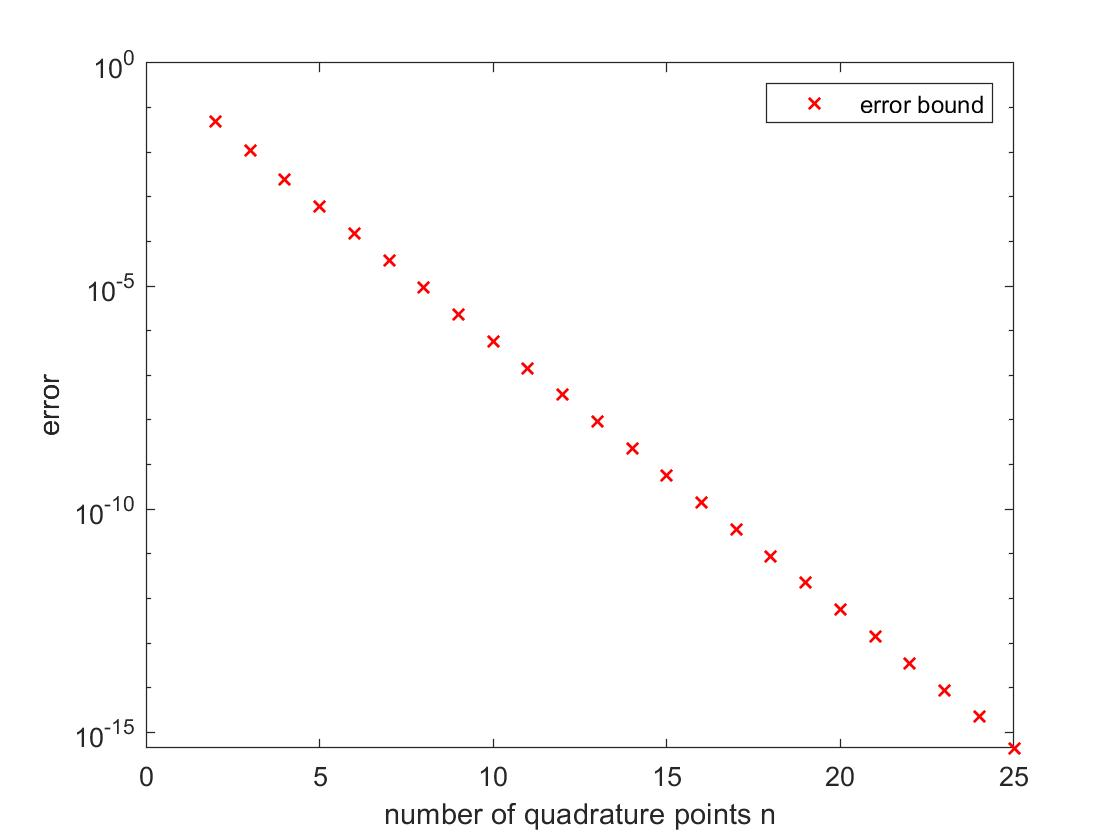
\includegraphics[width = .8\textwidth]{1a.jpg}
    \caption{误差随迭代次数变化}
\end{figure}

\subitem(b)
\textsc{Matlab}程序如下:
\begin{lstlisting}[frame=single]
clear, clc, clf
LW = 'linewidth'; lw = 1;
format long

MAX_ITER = 30;
a = -1; b = 1;
epsilon = 1e-15;
R_kj = zeros(MAX_ITER, MAX_ITER);
error_bound = zeros(MAX_ITER);

h = b - a;
k = (1 : MAX_ITER);
h_k = h ./ (2 .^ (k - 1));


R_kj(1,1) = (Func(a) + Func(b)) * h / 2;
count = 2;
for k = 2 : MAX_ITER
    for i = 1 : 2^(k-2)
        R_kj(k,1) = R_kj(k,1) + Func(a+(2*i-1)*h_k(k));
        count = count + 1;
    end
    R_kj(k,1) = (R_kj(k-1,1) + h_k(k-1) * R_kj(k,1))/2;
    
    for j = 2:k
        R_kj(k,j) = R_kj(k,j-1) + ...
        (R_kj(k,j-1) - R_kj(k-1,j-1)) / (4^(j-1)-1);
    end

    error_bound(k) = abs(R_kj(k,k) - R_kj(k-1,k-1));
    if error_bound(k) < epsilon
        break
    end
end
count
R_kj(k,k)

iter = 1 : MAX_ITER;
semilogy(iter, error_bound, 'rx', LW, lw)
xlabel('number of quadrature points n')
ylabel('error')
legend('error', 'location', 'ne')

function y = Func(x)
    y = sin(cos(sin(cos(x))));
end
\end{lstlisting}

输出结果:$1.339880713117284$,共计使用$257$个积分点。

误差变化:

\begin{figure}[H]
    \centering
    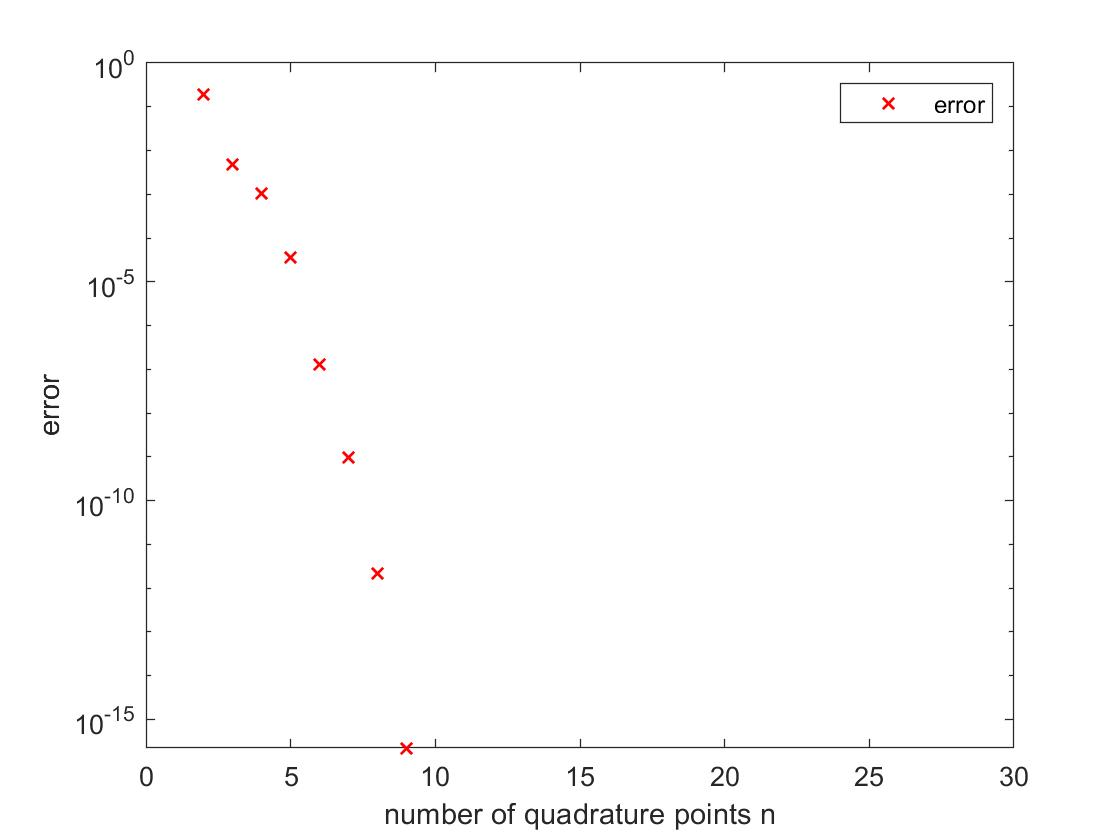
\includegraphics[width = .8\textwidth]{1b.jpg}
    \caption{误差随迭代次数变化}
\end{figure}

\subitem(c)
\textsc{Matlab}程序如下:
\begin{lstlisting}[frame=single]
clear, clc, clf
LW = 'LineWidth'; lw = 2;
MS = 'MarkerSize'; ms = 20;
format long

F = @(x)(sin(cos(sin(cos(x)))));
N = 30;
epsilon = 1e-15;
AbsErr = zeros(N, 1);
Integrate = zeros(N,1);
count = 0;
for n = 1 : N
    [x, w] = gauss(n);
    Integrate(n) = w*F(x);
    count = count + length(x);
    if n > 1
        AbsErr(n) = abs(Integrate(n) - Integrate(n-1));
        if AbsErr(n) < epsilon
            break
        end
    end
end
count
Integrate(n)

nvec = 1:N; % number of the quadrature points
semilogy(nvec, AbsErr, '.', MS, ms)
xlabel('number of quadrature points n')
ylabel('error')
legend('absolute Error')

% GAUSS  nodes x (Legendre points) and weights w
%        for Gauss quadrature
function [x,w] = gauss(N)
    beta = .5 ./ sqrt(1 - (2 * (1:N-1)).^(-2));
    T = diag(beta,1) + diag(beta,-1);
    [V,D] = eig(T);
    x = diag(D); [x,i] = sort(x);
    w = 2 * V(1,i).^2;
end
\end{lstlisting}

输出结果:$1.339880713117285$,共计使用$136$个积分点。

误差变化:

\begin{figure}[H]
    \centering
    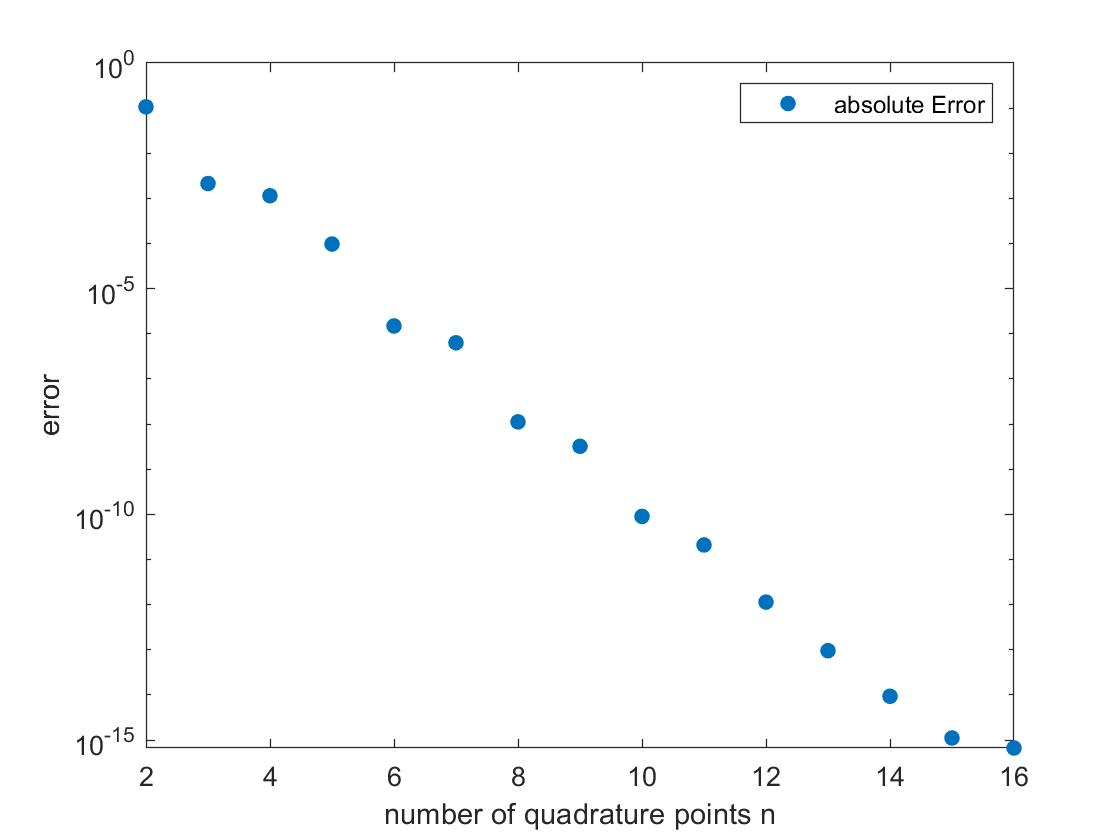
\includegraphics[width = .8\textwidth]{1c.jpg}
    \caption{误差随迭代次数变化}
\end{figure}

\subitem(d)
由前述程序输出可知,三种方法分别使用了$16777217$,$257$,$136$个积分点,到达$1e-15$的精度。效率依次递增。

\item[第二题] \textbf{函数求导与微分矩阵} 
\subitem(a)
由题,
\begin{equation}
    \ell_j(x) = \frac{1}{\pi_j} \prod_{k=0\\k \neq j}^{n}(x-x_k)
\end{equation}
故
\begin{equation}
    \begin{aligned}
        \ell_j^{'}(x) &= \frac{1}{\pi_j} \sum_{\substack{t=0\\t \neq j}}^{n} \sum_{\substack{k=0\\k \neq t\\k \neq j}}^{n} (x-x_k)\\
        &= \frac{1}{\pi_j} \prod_{\substack{t=0\\t \neq j}}^{n} (x-x_t) \cdot \sum_{\substack{k=0\\k \neq j}}^{n} \frac{1}{x-x_k}\\
        &= \ell_j(x) \sum_{\substack{k=0\\k \neq j}}^{n} (x-x_k)^{-1}
    \end{aligned}
\end{equation}

\subitem(b)
\textsc{Matlab}程序如下:
\begin{lstlisting}[frame=single]
clear, clc, clf
LW = 'linewidth'; lw = 1;

n = 15;
x = linspace(-1, 1, n + 1)';
m = 1000;
xx = linspace(-1, 1, m + 1)';
F = @(x)(sin(x));
dF = @(x)(cos(x));
exact = dF(xx);

pi_j = ones(n + 1, 1);
for j = 1 : n + 1
    for k = 1 : n + 1
        if k ~= j
            pi_j(j) = pi_j(j) * (x(j) - x(k));
        end
    end
end

f_j = F(x);

l_j = ones(m + 1, n + 1);
for i = 1 : m + 1
    for j = 1 : n + 1
        loc_sum = 0;
        for k = 1 : n + 1
            if k ~= j
                l_j(i, j) = l_j(i, j) * (xx(i)-x(k));
                loc_sum = loc_sum + 1/(xx(i)-x(k));
            end
        end
        l_j(i, j) = l_j(i, j) * loc_sum / pi_j(j);
    end
end

dp = l_j * f_j;

figure(1)
plot(xx, exact, 'k', LW, lw), hold on
plot(xx, dp, 'r:', LW, lw)
xlabel('x')
ylabel('y')
legend('exact', 'interpolant', 'location', 'se')

figure(2)
plot(2)
semilogy(xx, abs(exact - dp), 'k', LW, lw)
xlabel('x')
ylabel('error')
legend('error', 'location', 'ne')
\end{lstlisting}

程序输出插值得到的导函数:

\begin{figure}[H]
    \centering
    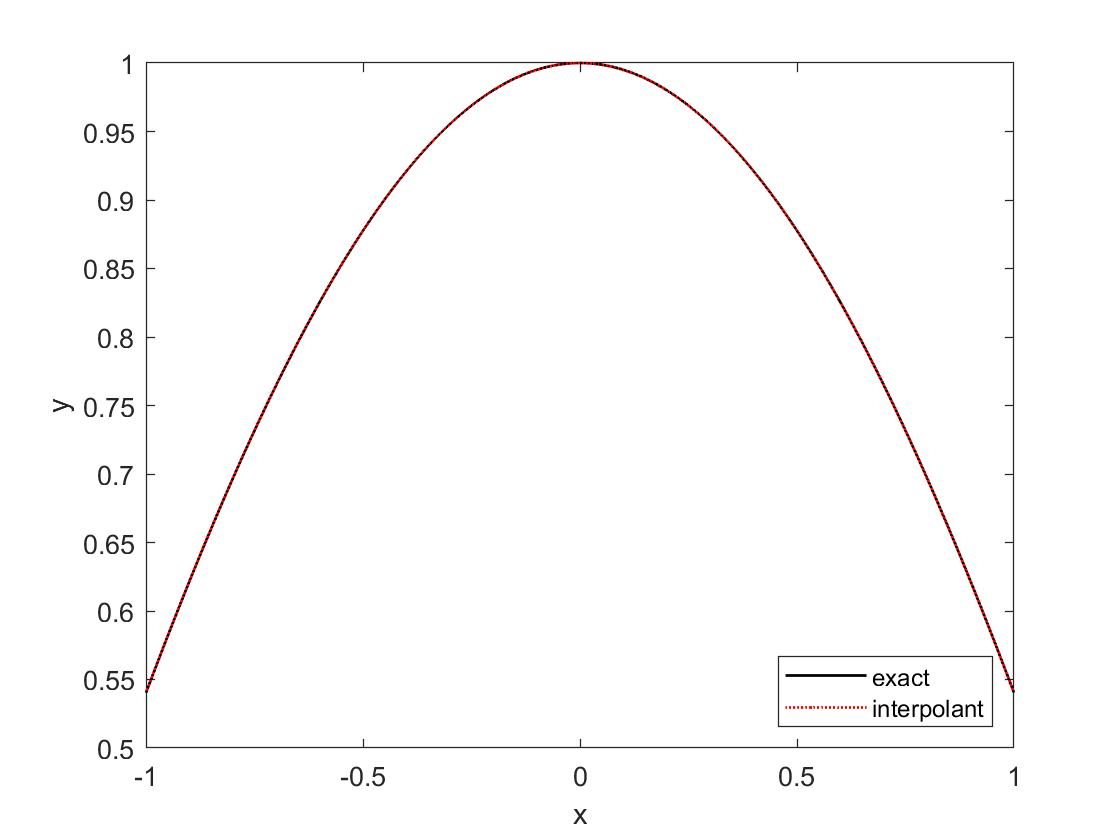
\includegraphics[width = .8\textwidth]{2b_interp.jpg}
    \caption{导函数}
\end{figure}

误差绝对值:

\begin{figure}[H]
    \centering
    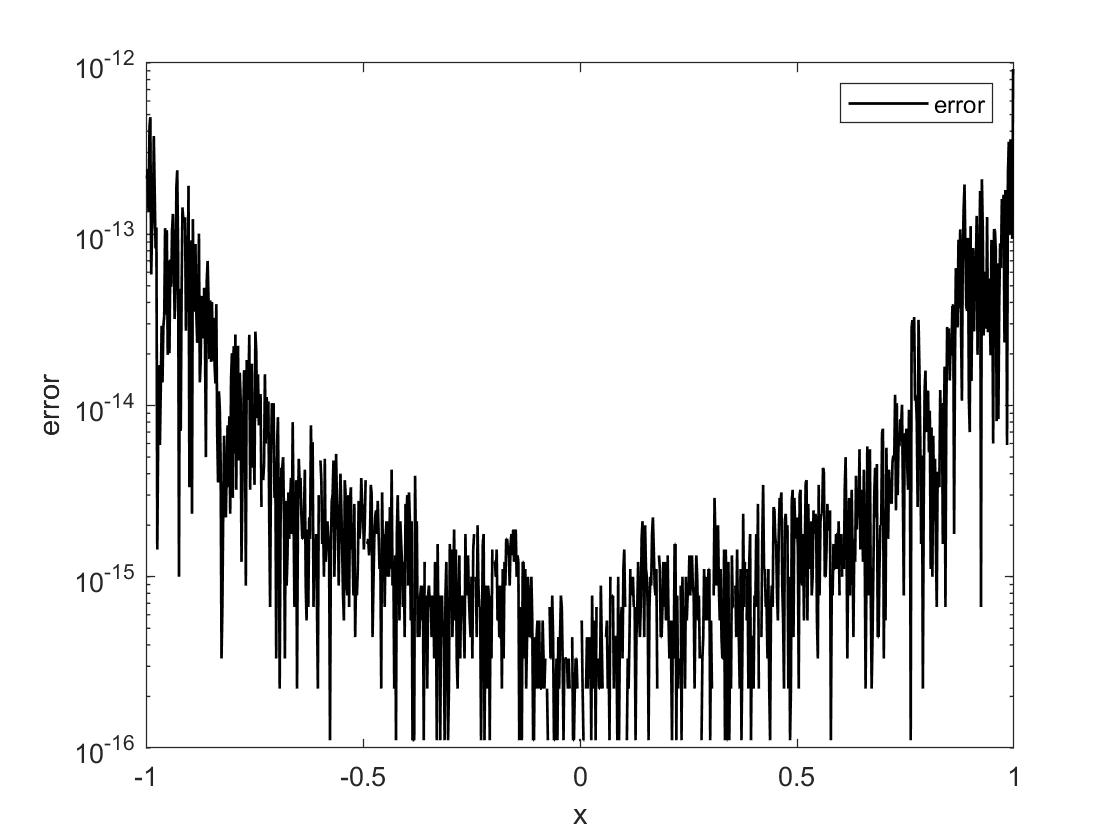
\includegraphics[width = .8\textwidth]{2b_error.jpg}
    \caption{误差}
\end{figure}

\subitem(c)
由$p^{'}(x)$写成矩阵相乘形式\\
记$S_j(x) = \sum_{\substack{k=0\\k \neq j}}^{n} \frac{1}{x-x_k}$,有
\begin{equation}
    \begin{aligned}
        p^{'}(x) &= \sum_{j=0}^{n} f(x_j)\ell_j(x)S_j(x) \\
        &= \begin{pmatrix}
            \ell_0(x)S_0(x) & \ell_1(x)S_1(x) & \cdots & \ell_n(x)S_n(x)
        \end{pmatrix} \cdot \begin{pmatrix}
            f(x_0) \\
            f(x_1) \\
            \vdots \\
            f(x_n)
        \end{pmatrix}
    \end{aligned}
\end{equation}

令
\begin{equation}
    \mathbf{P^{'}} = \begin{pmatrix}
        p^{'}(x_0)\\
        \vdots \\
        p^{'}(x_n)
    \end{pmatrix} = \begin{pmatrix}
        D_{00} & \cdots & D_{0n} \\
        \vdots & \ddots & \vdots \\
        D_{n0} & \cdots & D_{nn}
    \end{pmatrix} \cdot \begin{pmatrix}
        f(x_0) \\
        \vdots \\
        f(x_n)
    \end{pmatrix}
\end{equation}

则有$D_{ij} = \ell_j(x_i)S_j(x_i)$.\\
$i = j$时,$\ell_j(x_j) = 1$,$D_{ij} = S_j(x_j) = \sum_{\substack{k=0\\k \neq j}}^{n} (x_j-x_k)^{-1}$\\
$i \neq j$时,
\begin{equation}
    \begin{aligned}
        D_{ij} &= \frac{1}{\pi_j} \left(\prod_{\substack{k=0\\k \neq j}}^{n}(x_i-x_k)\right) \left(\sum_{\substack{t=0\\t \neq j}}^{n} (x_i-x_t)^{-1}\right) \\
        &= \frac{1}{\pi_j} \sum_{\substack{t=0\\t \neq j}}^{n} \frac{x_i-x_t}{x_i-x_t} \prod_{\substack{k=0\\k \neq j\\k \neq t}}^{n} (x_i-x_k) \\
        &= \frac{1}{\pi_j} \sum_{\substack{t=0\\t \neq j}}^{n} \left(\prod_{\substack{k=0\\k \neq j\\k \neq t}}^{n} (x_i-x_k) \right)\\
        &= \frac{1}{\pi_j} \prod_{\substack{t=0\\t \neq j}}^{n} (x_i-x_k) \\
        &= \frac{\pi_i}{\pi_j(x_i-x_j)}
    \end{aligned} \nonumber
\end{equation}

\subitem(d)
\textsc{Matlab}程序如下:
\begin{lstlisting}[frame=single]
clear, clc, clf
LW = 'linewidth'; lw = 1;

F = @(x)(sin(3 .* x .^ 2));
dF = @(x)(6 .* x .* cos(3 .* x .^ 2));

MAX_ITER = 30;
iter_n = 2 * (1:MAX_ITER)' - 1;
max_error1 = zeros(MAX_ITER, 1);
max_error2 = zeros(MAX_ITER, 1); % Chebyshev error

for iter = 1:MAX_ITER
    n = 2 * iter - 1;
    x1 = linspace(-1, 1, n + 1)';
    % Chebyshev
    x2 = (0:n)';
    x2 = cos(x2 .* pi ./ n);
    
    pi1_j = ones(n + 1, 1);
    pi2_j = ones(n + 1, 1);
    for j = 1 : n + 1
        for k = 1 : n + 1
            if k ~= j
                pi1_j(j) = pi1_j(j) * (x1(j) - x1(k));
                pi2_j(j) = pi2_j(j) * (x2(j) - x2(k));
            end
        end
    end

    D1_ij = zeros(n+1, n+1);
    D2_ij = zeros(n+1, n+1);
    for i = 1:n+1
        for j = 1:n+1
            if i == j
                for k = 1:n+1
                    if k ~= j
                        D1_ij(i,j) = D1_ij(i,j) +...
                        1/(x1(j)-x1(k));
                        D2_ij(i,j) = D2_ij(i,j) +...
                        1/(x2(j)-x2(k));
                    end
                end
            else
                D1_ij(i,j) = pi1_j(i)/(pi1_j(j) *...
                (x1(i)-x1(j)));
                D2_ij(i,j) = pi2_j(i)/(pi2_j(j) *...
                (x2(i)-x2(j)));
            end
        end
    end

    f1_j = F(x1);
    f2_j = F(x2);

    dp1 = D1_ij * f1_j;
    dp2 = D2_ij * f2_j;

    exact1 = dF(x1);
    exact2 = dF(x2);

    max_error1(iter) = max(abs(dp1 - exact1));
    max_error2(iter) = max(abs(dp2 - exact2));
end

figure(1)
semilogy(iter_n, max_error1, 'k', LW, lw), hold on
semilogy(iter_n, max_error2, 'r:', LW, lw)
xlabel('x')
ylabel('error')
legend('error1', 'error2(cheby)', 'location', 'sw')
\end{lstlisting}

逐点误差绝对值的最大值随n变化的情况:

\begin{figure}[H]
    \centering
    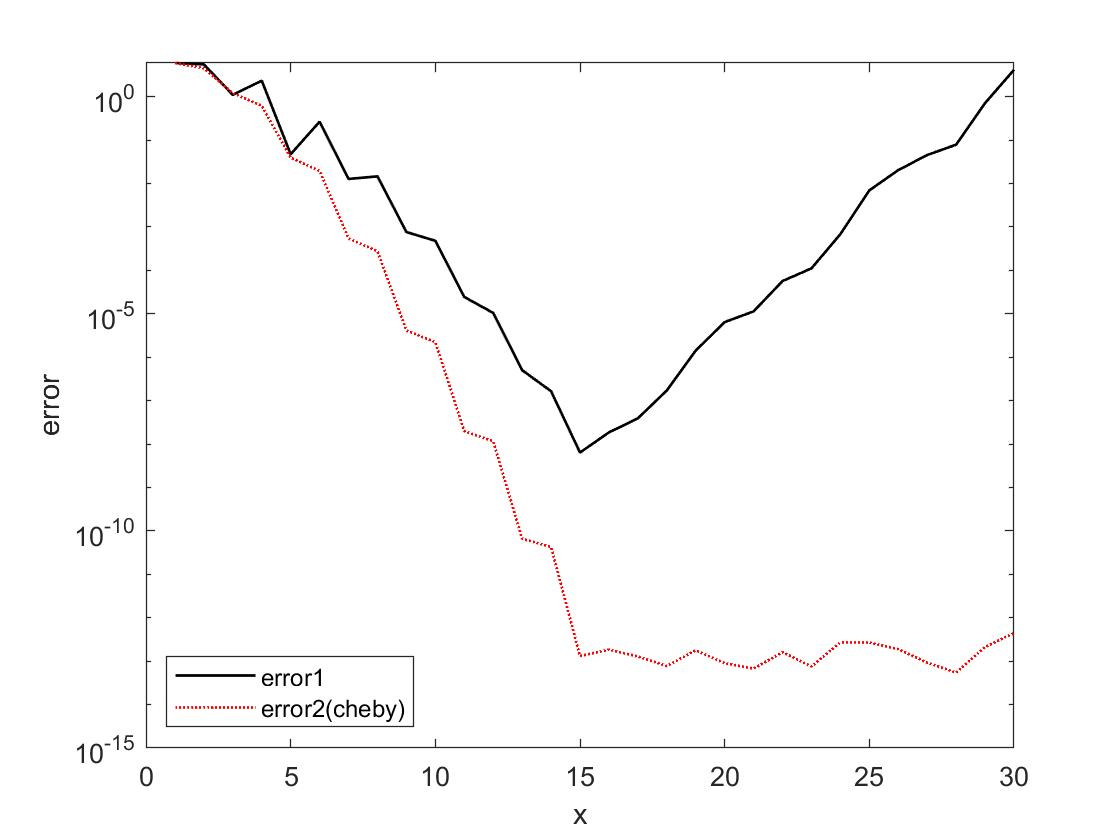
\includegraphics[width = .8\textwidth]{2d.jpg}
    \caption{逐点误差绝对值的最大值随n变化的情况}
\end{figure}

\item[第三题]
\subitem(a)
由于公式右端出现$f_{n+1}$,所以该公式是隐式格式。且从下式可知$p=1,q=3$.
\begin{equation}
    \begin{aligned}
        y_{n+1} = y_{n-p} +& \int_{x_{n-p}}^{x_{n+1}}L_{n+1-q}^{n+1}(x) \mathrm{d}x\\
        =y_{n-1} +& 
        f_{n+1}\int_{x_{n-1}}^{x_{n+1}} \frac{(x-x_{n})(x-x_{n-1})(x-x_{n-2})}{(x_{n+1}-x_{n})(x_{n+1}-x_{n-1})(x_{n+1}-x_{n-2})}\mathrm{d}x\\
         +& f_n\int_{x_{n-1}}^{x_{n+1}} \frac{(x-x_{n+1})(x-x_{n-1})(x-x_{n-2})}{(x_n-x_{n+1})(x_n-x_{n-1})(x_n-x_{n-2})}\mathrm{d}x\\
         +& f_{n-1}\int_{x_{n-1}}^{x_{n+1}} \frac{(x-x_{n+1})(x-x_{n})(x-x_{n-2})}{(x_{n-1}-x_{n+1})(x_{n-1}-x_{n})(x_{n-1}-x_{n-2})}\mathrm{d}x\\
         +& f_{n-2}\int_{x_{n-1}}^{x_{n+1}} \frac{(x-x_{n+1})(x-x_{n})(x-x_{n-1})}{(x_{n-2}-x_{n+1})(x_{n-2}-x_{n})(x_{n-2}-x_{n-1})}\mathrm{d}x\\
        =y_{n-1} +& \frac{1}{3}hf_{n+1}+\frac{4}{3}hf_n+\frac{1}{3}hf_{n-1}
    \end{aligned}
\end{equation}

由此可得
\begin{equation}
    \left\{\begin{array}{l}
        \alpha=\frac{1}{3}h \\
        \beta=\frac{4}{3}h \\
        \gamma=\frac{1}{3}h \\
        \mu=0
    \end{array}\right.
\end{equation}

\subitem(b)
若$y_n=y(x_n),y_{n-1}=y(x_{n-1})$,则$y(x_{n+1})$的局部截断误差为
\begin{equation}
    \begin{aligned}
        T_{n+1}=&y(x_{n+1})-y_{n+1}\\
        =&y(x_{n+1})-(y_{n-1}+\frac{1}{3}hf_{n+1}+\frac{4}{3}hf_n+\frac{1}{3}hf_{n-1})\\
        =&y(x_{n+1})-(y_{n-1}+\frac{1}{3}hy^{'}_{n+1}+\frac{4}{3}hy^{'}_n+\frac{1}{3}hy^{'}_{n-1})
    \end{aligned}
\end{equation}

将$y(x_{n+1})$在$y(x_{n-1})$处作泰勒展开
\begin{equation}
    \begin{aligned}
        y(x_{n+1})=&y(x_{n-1}+2h)\\
        = &y(x_{n-1})+2hy^{'}(x_{n-1})+\frac{(2h)^2}{2!}y^{''}(x_{n-1})+\frac{(2h)^3}{3!}y^{(3)}(x_{n-1})\\
        &+\frac{(2h)^4}{4!}y^{(4)}(x_{n-1})+\frac{(2h)^5}{5!}y^{(5)}(x_{n-1})+\frac{(2h)^6}{6!}y^{(6)}(\xi_1)
    \end{aligned}
\end{equation}

将$y^{'}(x_{n+1})$在$y^{'}(x_{n-1})$处作泰勒展开
\begin{equation}
    \begin{aligned}
        y^{'}(x_{n+1})=&y^{'}(x_{n-1}+2h)\\
        =&y^{'}(x_{n-1})+2hy^{''}(x_{n-1})+\frac{(2h)^2}{2!}y^{(3)}(x_{n-1})+\frac{(2h)^3}{3!}y^{(4)}(x_{n-1})\\
        &+\frac{(2h)^4}{4!}y^{(5)}(x_{n-1})+\frac{(2h)^5}{5!}y^{(6)}(x_{n-1})+\frac{(2h)^6}{6!}y^{(7)}(\xi_2)
    \end{aligned}
\end{equation}

将$y^{'}(x_n)$在$y^{'}(x_{n-1})$处作泰勒展开
\begin{equation}
    \begin{aligned}
        y^{'}(x_{n})=&y^{'}(x_{n-1}+h)\\
        =&y^{'}(x_{n-1})+hy^{''}(x_{n-1})+\frac{h^2}{2!}y^{(3)}(x_{n-1})+\frac{h^3}{3!}y^{(4)}(x_{n-1})\\&+
        \frac{h^4}{4!}y^{(5)}(x_{n-1})+\frac{h^5}{5!}y^{(6)}(x_{n-1})+\frac{h^6}{6!}y^{(7)}(\xi_3)
    \end{aligned}
\end{equation}

将以上三式代入$T_{n+1}$:
\begin{equation}
    \begin{aligned}
        T_{n+1}=&y(x_{n+1})-(y_{n-1}+\frac{1}{3}hy^{'}_{n+1}+\frac{4}{3}hy^{'}_n+\frac{1}{3}hy^{'}_{n-1})\\
        =&y(x_{n-1})-y_{n-1}\\
        &+y^{'}(x_{n-1})\Big( 2h-\frac{1}{3}h-\frac{4}{3}h-\frac{1}{3}h \Big)\\
        &+y^{''}(x_{n-1})\Big[ \frac{(2h)^2}{2!}-\frac{1}{3}h\cdot2h-\frac{4}{3}h \Big]\\
        &+y^{(3)}(x_{n-1})\Big[\frac{(2h)^3}{3!}-\frac{1}{3}h\cdot\frac{(2h)^2}{2!}-\frac{4}{3}h\cdot\frac{h^2}{2!}\Big]\\
        &+y^{(4)}(x_{n-1})\Big[\frac{(2h)^4}{4!}-\frac{1}{3}h\cdot\frac{(2h)^3}{3!}-\frac{4}{3}h\cdot\frac{h^3}{3!}\Big]\\
        &+y^{(5)}(x_{n-1})\Big[\frac{(2h)^5}{5!}-\frac{1}{3}h\cdot\frac{(2h)^4}{4!}-\frac{4}{3}h\cdot\frac{h^4}{4!}\Big]\\
        &+O(h^6)\\
        =&-\frac{1}{90}h^5y^{(5)}(x_{n-1})+O(h^6)\\
        =&O(h^5)
    \end{aligned}
\end{equation}
故该多步格式是4阶的。

\subitem(c)
起步计算需要计算$y_0$,$y_1$.\\
取步长$h=0.1$,计算公式为
\begin{equation}
    \left\{\begin{array}{l}
        y_{n+1}=y_n+\frac{h}{6}(k_1+4k_2+k_3)\\
        k_1=x_n\mathrm{e}^{-5x_n}-5y_n\\
        k_2=(x_n+\frac{1}{2}h)\mathrm{e}^{-5(x_n+\frac{1}{2}h)}-5(y_n+\frac{1}{2}hk_1)\\
        k_3=(x_n+h)\mathrm{e}^{-5(x_n+h)}-5(y_n-hk_1+2hk_2)
    \end{array}\right.
\end{equation}

起步计算结果:

\begin{center}
    \begin{tabular}{c|c|c}
        \hline
        $n$ & $x_n$ & $y_n$ \\
        \hline
        0 & 0   & 0\\
        1 & 0.1 & 0.002957886390533\\
        \hline
    \end{tabular}
\end{center}

多步格式计算结果:

\begin{center}
    \begin{tabular}{c|c|r}
        \hline
        $n$ & $x_n$ & $y_n$ \\
        \hline
        2 & 0.2 & 0.007343726408820\\
        3 & 0.3 & 0.009970522815425\\
        4 & 0.4 & 0.010847111360544\\
        5 & 0.5 & 0.010195395534566\\
        6 & 0.6 & 0.009012749282441\\
        7 & 0.7 & 0.007322843843022\\
        8 & 0.8 & 0.005941122311851\\
        9 & 0.9 & 0.004399855987501\\
        10 & 1.0 & 0.003483250962686\\
        11 & 1.1 & 0.002336477539911\\
        12 & 1.2 & 0.001944170491693\\
        13 & 1.3 & 0.001082184532716\\
        14 & 1.4 & 0.001115131223007\\
        15 & 1.5 & 0.000361217867742\\
        16 & 1.6 & 0.000736737268505\\
        17 & 1.7 & -0.000068051859298\\
        18 & 1.8 & 0.000626340904567\\
        19 & 1.9 & -0.000367184265150\\
        20 & 2.0 & 0.000682400552320\\
        \hline
    \end{tabular}
\end{center}

使用三阶的Runge-Kutta方法作为起步方法时,计算$y_1$的截断误差是$O(h^4)$,而四阶多步格式的整体截断误差也是$O(h^4)$。两个$O(h^4)$相加仍然是$O(h^4)$,所以不影响精度。

\subitem(d)
推导精确解:
\begin{equation}
    \begin{aligned}
        y^{'}(x)+5y(x)&=x\mathrm{e}^{-5x}\\
        \mathrm{e}^{5x}y^{'}(x)+5\mathrm{e}^{5x}y(x)&=x\\
        \frac{\mathrm{d}}{\mathrm{d}x}(\mathrm{e}^{5x}y(x))&=x\\
        \mathrm{e}^{5x}y(x)&=\frac{1}{2}x^2+\text{Const}\\
        y(x)&=\frac{1}{2}\mathrm{e}^{-5x}x^2
    \end{aligned}
\end{equation}

\textsc{Matlab}程序验证多步格式的四阶精度:
\begin{lstlisting}[frame=single]
clear, clc, clf
LW = 'linewidth'; lw = 2;
f = @(x)(x.^2.*exp(-5.*x)./2);
H = 10.^-(1:0.1:3);
err = zeros(length(H), 1);

for i = 1:length(H)
    h = H(i);
    xn = (0:h:2)';
    exact = f(xn);

    x = xn(1);
    yn = zeros(length(xn), 1);
    k1 = x * exp(-5 * x) - 5 * yn(1);
    k2 = (x+h/2) * exp(-5 * (x+h/2)) - 5*(yn(1)+h/2*k1);
    k3 = (x+h) * exp(-5*(x+h)) - 5*(yn(1)-h*k1+2*h*k2);
    yn(2) = yn(1) + h/6*(k1+4*k2+k3);

    for k = 3:length(yn)
        yn(k) = ( yn(k-2) + ...
        h/3*(xn(k)*exp(-5*xn(k))) + ...
        4*h/3*(xn(k-1)*exp(-5*xn(k-1))-5*yn(k-1)) + ...
        h/3*(xn(k-2)*exp(-5*xn(k-2))-5*yn(k-2)) ) / ...
        (1+5*h/3);
    end

    err(i) = abs(yn(end) - f(xn(end)));
end

loglog(H, err, '.', LW, lw)
xlabel('h')
ylabel('error')
legend('error', 'location', 'se')
\end{lstlisting}

运行结果:

\begin{figure}[H]
    \centering
    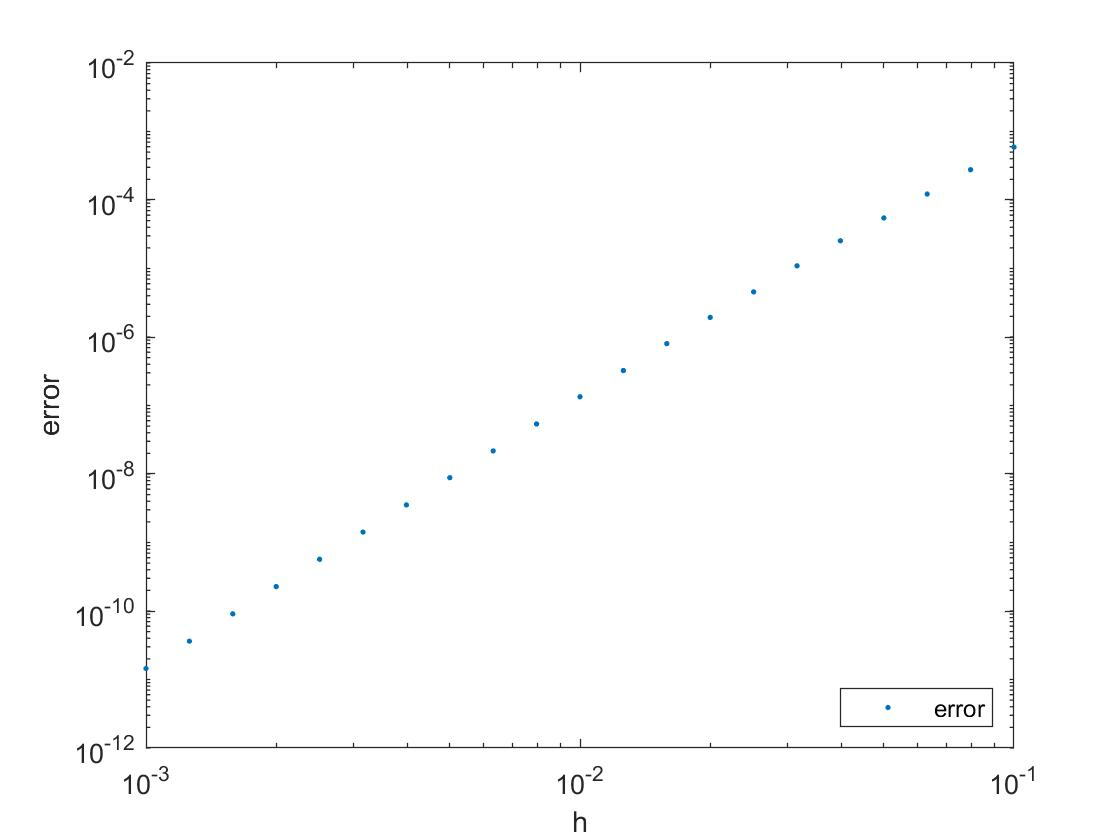
\includegraphics[width = .8\textwidth]{3.jpg}
    \caption{截断误差随步长变化}
\end{figure}
图象斜率为$4$,符合前述推断。

\end{enumerate}

\end{document}
